\documentclass[a4paper, 14pt]{article}
\usepackage[T2A]{fontenc}
\usepackage[utf8]{inputenc}
\usepackage[english,russian]{babel}
\usepackage[top = 2cm, bottom = 2 cm]{geometry}
\usepackage{cmap}
\usepackage{graphicx}
\usepackage{listings}
\usepackage{color}
\usepackage{amsmath}
\usepackage{pgfplots}
\usepackage{url}
\usepackage{tikz}
\usepackage{float}
\usepackage{multirow}

\usepackage{titlesec}
\titleformat*{\section}{\LARGE\bfseries}
\titleformat*{\subsection}{\Large\bfseries}
\titleformat*{\subsubsection}{\large\bfseries}
\titleformat*{\paragraph}{\large\bfseries}
\titleformat*{\subparagraph}{\large\bfseries}


\begin{document}

	\textbf{Цель работы:} реализовать программу для построения графиков функции и плотности следующих распределений:
\begin{itemize}
\item равномерное распределение;
\item распределение Эрланга. 
\end{itemize}
	
	
	\section*{Равномерное распределение}
	
Равномерное распределение - распределение случайной величины, принимающей значения, принадлежащие некоторому промежутку конечной длины, характеризующееся тем, что плотность вероятности на этом промежутке всюду постоянна.\\

Функция распределения:

\begin{equation*}
F_X (x) =
    \begin{cases}
        0, x < a \\
        \frac{x - a}{b - a}, a \le x < b \\
        1, x \geq b \\
    \end{cases}
\end{equation*}
	
Плотность распределения:

\begin{equation*}
    f_X (x) =
    \begin{cases}
        \frac{1}{b-a}, x \in [a,b] \\
        0, x \notin [a, b] \\
    \end{cases}
\end{equation*}


\section*{Распределение Эрланга}

Распределение Эрланга – это гамма-распределение  с параметром $k$, принимающим лишь целые значения. \\

Функция распределения:

\begin{equation*}
F_X(x) = 1 - \sum_{i=0}^k  \frac{1}{i!} e^{-\lambda x} (\lambda x)^n
\end{equation*}
	
Плотность распределения:

\begin{equation*}
f_X(x) = \frac{\lambda^k x^{k-1} e^{-\lambda x} } {(k-1)!}
\end{equation*}


\section*{Результаты работы}

\begin{figure}[H]
    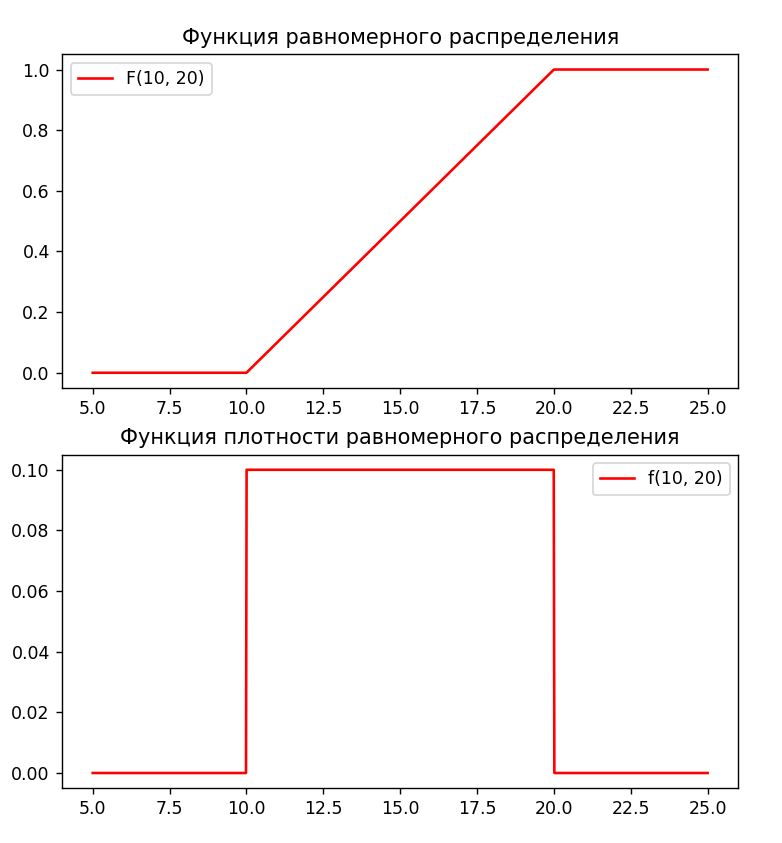
\includegraphics[scale=0.4]{1}
    \caption{Равномерное распределение при $a=-3$, $b=3$}
    \label{fig:}
\end{figure}

\begin{figure}[H]
    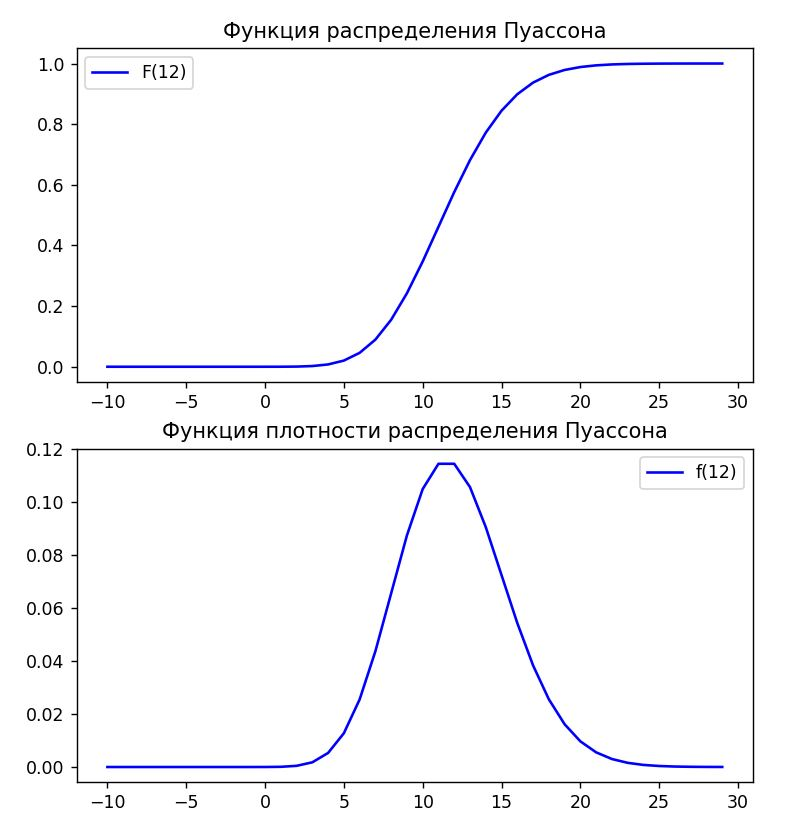
\includegraphics[scale=0.4]{2}
    \caption{Равномерное распределение при $a=0$, $b=8$}
    \label{fig:}
\end{figure}

\begin{figure}[H]
    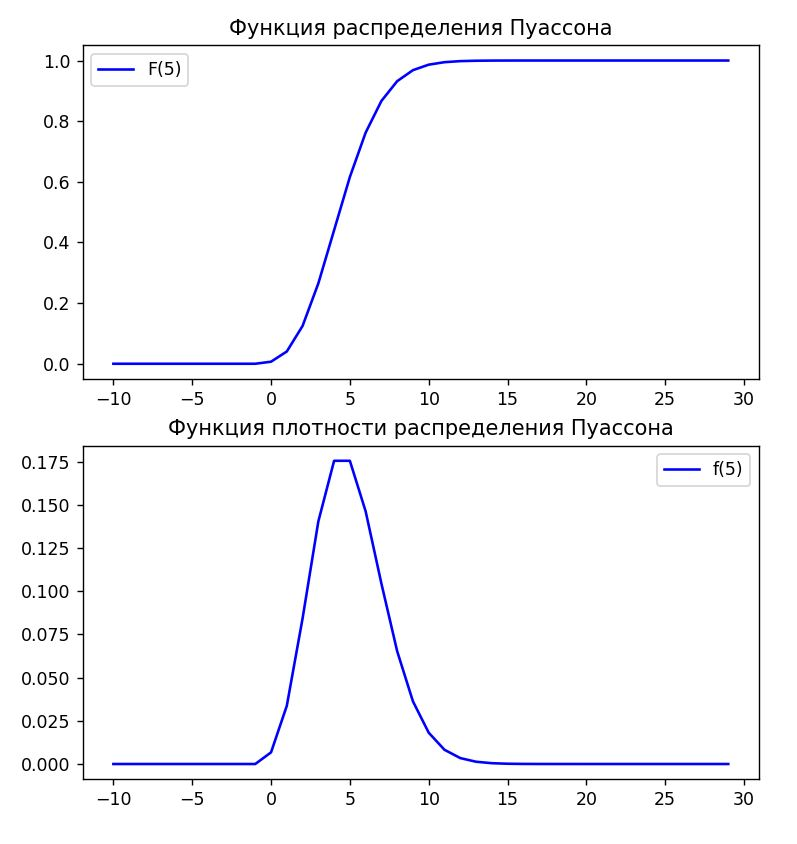
\includegraphics[scale=0.4]{3}
    \caption{Распределение Эрланга при $\lambda=3$, $k=3$}
    \label{fig:}
\end{figure}

\begin{figure}[H]
    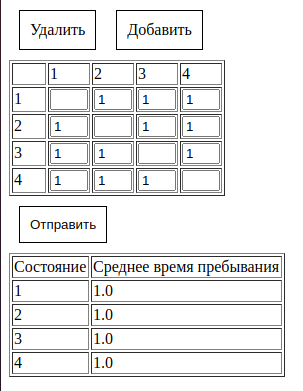
\includegraphics[scale=0.4]{4}
    \caption{Распределение Эрланга при $\lambda=4$, $k=2$}
    \label{fig:}
\end{figure}

\section*{Вывод}
В ходе выполнения лабораторной работы была реализована программа для построения графиков функции и плотности равномерного распределения и распределения Эрланга. Были построены графики при различных параметрах $a, b$ для равномерного распределения и $\lambda, k$ для распределения Эрланга.
\end{document}